\documentclass[14pt]{beamer}
\usepackage{beamerthemeshadow}
%\usepackage{beamerthemesidebar}
\usepackage{graphicx}

%\usepackage{polski}
%\usepackage[latin2]{inputenc}


\newcommand{\net}[0]{{\tt .NET}}
\newcommand{\kw}[1]{{\textcolor{kwcolor}{\tt #1}}}

\definecolor{kwcolor}{rgb}{0.2,0.4,0.0}
\definecolor{lgray}{rgb}{0.8,0.8,0.8}

\title{Nemerle}
\author{Micha{\l} Moskal, Kamil Skalski, Pawe{\l} Olszta}
\institute{Computer Science Institute, University of Wroc{\l}aw}
\date{\today}



\begin{document}

\section{Introduction}

\frame{\titlepage}

\frame{
\frametitle{Nemerle features}
\begin{itemize}
  \item functional programming language
  \item since the beginning designed for the \net
  \item imperative and object oriented
  \item Turing-complete macros
  \item assertion system
\end{itemize}
}


\frame{
\frametitle{Why \net\ ?}

\begin{itemize}
  \item wide variety of libraries
  \item runtime environment (GC, JIT)
  \item portable executable files (Microsoft \net, Mono, DotGNU, Rotor)
  \item dynamic class loading
  \item dynamic code generation
\end{itemize}
}

\frame{
\frametitle{Why new language?}

\begin{itemize}
  \item ports of existing languages are cut-down in the best case
  \item ease of definition vs ease of use
  \item easy access to imperative features
  \item simple object oriented system (directly from \net)
\end{itemize}
}

\frame{
\frametitle{Theory vs industry}
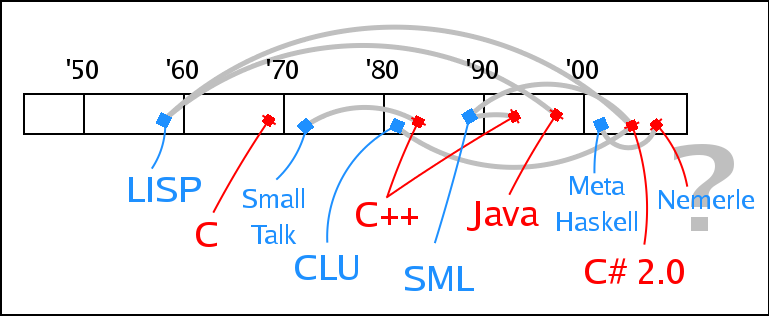
\includegraphics[width=1.0\textwidth]{years}
}

\frame{
\frametitle{What about the language?}

\begin{itemize}
  \item syntax reassembles C\#, especially at the class and method level
  \item expressions syntactically from C, semantically from ML
  \begin{itemize}
    \item no statements -- just expressions
    \item pattern matching on variant types
    \item functions as first class citizens
  \end{itemize}
\end{itemize}
}


\section{We all like examples}

\frame[containsverbatim]{
\frametitle{Hello}

\begin{verbatim}
class Hello {
  public static Main () : void {
    System.Console.Write ("Hello world!\n")
  }
}
\end{verbatim}
}


\frame[containsverbatim]{
\frametitle{Factorial}
\begin{verbatim}
module Factorial {
  public factorial (x : int) : int {
    def loop (acc : int, x : int) : int {
      if (x <= 1) acc
      else loop (acc * x, x - 1)
    };
    loop (1, x)
  }
}
\end{verbatim}
}

\frame[containsverbatim]{
\frametitle{Lists}
\begin{verbatim}
variant list <'a> {
  | Cons { hd : 'a; tl : list ('a); }
  | Nil
}
head<'a> (x : list <'a>) : 'a {
  match (x) {
    | Cons (x, _) => x
    | Nil => 
      throw InvalidArgumentException ()
  }
}
\end{verbatim}
}

\frame[containsverbatim]{
\frametitle{Trees}
\begin{verbatim}
interface IComparable <'a> {
  compare (other : 'a) : int;
}

variant tree <'a> 
  where 'a : IComparable <'a> {
  | Node { left  : tree <'a>; 
           elem  : 'a; 
           right : tree <'a>; }
  | Tip
}
\end{verbatim}
}

\frame[containsverbatim]{
\frametitle{Variant inheritance}
\begin{verbatim}
class Located {
  public linenumber : int;
  public filename   : string;
}
variant Expression : Located {
  | E_ref { name : string; }
  | E_call { fn : Expression; 
             args : list <Expression>; }
}
\end{verbatim}
}


%\frame{
%\frametitle{Assertions}
%\begin{itemize}
%  \item \kw{require} and \kw{ensure}
%  \item \kw{ensure} pod koniec bloku (mo? korzysta栺 \kw{value})
%  \item zmienne strze?ne (\kw{guarded}, \kw{guard})
%  \begin{itemize}
%    \item zmiana $ \Rightarrow $ uruchomienie stra?ika
%    \item {\texttt{guarded x <- 3 \{ previous.x < x \};}}
%  \end{itemize}
%  \item \kw{transaction}
%\end{itemize}
%}

\section{Macros}
\frame{
\frametitle{Macros}
\begin{itemize}
  \item dynamically loaded compiler modules
  \item compilation-time or run-time execution
  \item written in Nemerle
  \item work on syntax trees of expressions and types
  \item can read external files, query database etc.
\end{itemize}
}


\frame{
\frametitle{Uses of macros}
\begin{itemize}
  \item specialized sublanguages ({\tt printf}, {\tt scanf}, regular expressions,
    SQL, XML, XPath)
  \item generation of syntax tress out of external files and {\it vice versa} 
       (Yacc, Burg, types from DTD, documentation generation)
  \item generating tress from other trees (serialization, specialization of code)
  \item interpreter implementation
\end{itemize}
}

\frame[containsverbatim]{
\frametitle{Example use of macro}
This macro checks syntax and type validness of query at compile-time
(by connecting to database). Creates code, which use {\tt SqlParameter}
to pass value of {\it myval} to {\tt SqlCommand} securely.

\begin{verbatim}
def myval = "Kate";
ExecuteReaderLoop ("SELECT * FROM employee WHERE"
                   " firstname = $myval", dbcon, 
{
  printf ("Name: %s %s\n", firstname, lastname)
});
\end{verbatim}
}


\section{Summary}
\frame{
\frametitle{Status}

\begin{itemize}
  \item compiler bootstraped
  \item 0.1 release, approaching 0.2
  \item standard library
  \item \net connectivity
  \item macros
  \item \textcolor{blue}{\tt http://nemerle.org/}
\end{itemize}
}

\frame{
\frametitle{TODO}

\begin{itemize}
  \item CLS extender (near!)
  \item take advantage of .NET generics
  \item further macro system development (AOP)
  \item better documentation
  \item formal definitions (semantics, type system, type inference)
\end{itemize}
}

\end{document}

% vim: language=english
